
\subsection{Debugging case study with Mininet}
\label{s:eval:mininet}
\label{sec:eval:mininet}

%TODO: Need a figure for this 4-host topology
To demonstrate \TheSystem's use in practice, we present a case study using
Mininet~\cite{mininet}.
%with a topology shown in Figure~\ref{fig:mininet-topo}.
Our topology consists of 4 hosts ({\ct h1, h2, h3, h4}) and 2 routers in a dumbbell topology.
One router is connected to {\ct h1} and {\ct h3}
and the other, to {\ct h2} and {\ct h4}.
The routers are connected via a single link and
programmed in \pfs~\cite{p4-bmv2} with queries compiled by \TheSystem.

Host {\ct h2} repeatedly downloads a 1MB objects over TCP from {\ct h1}.
Meanwhile, {\ct h3} sends {\ct h4} sporadic bursts of UDP traffic, which {\ct h4} acks.
Suppose a network admin notices the irregular latency
spikes for the TCP traffic (\Fig{mininet-latency}). She suspects a queue buildup
in the routers and measures the queue depths seen by the traffic by writing:
{\ct result = filter(\pktlog, srcip == h1 and dstip == h2).}

%%\begin{figure}[ht]
%%\centering
%%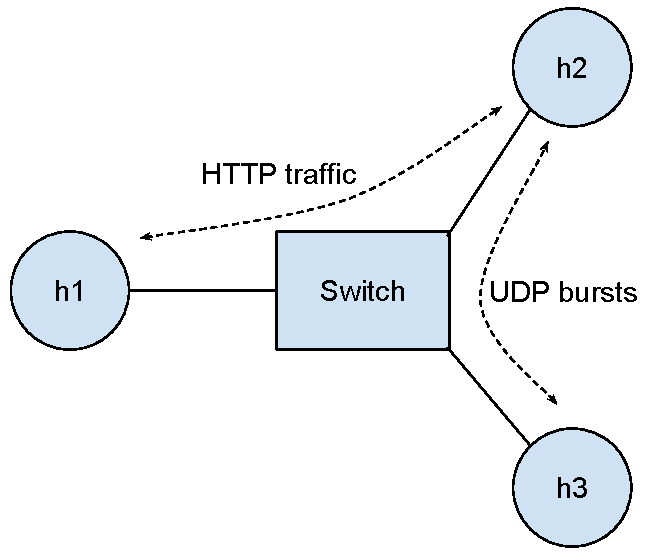
\includegraphics[width=0.4\columnwidth]{mininet-topo.pdf}
%%\caption{Mininet topology used for the case study.}
%%\label{fig:mininet-topo}
%%\end{figure}

\begin{figure}[!t]
\centering
\vspace{-0.1in}
\begin{subfigure}[t]{0.48\columnwidth}
\raggedright
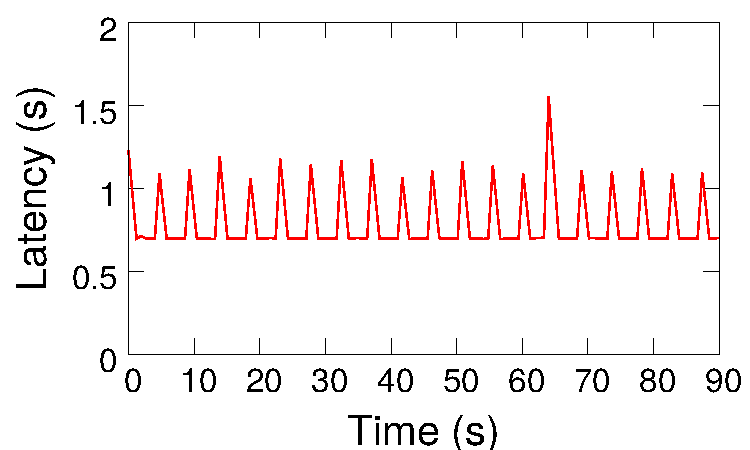
\includegraphics[width=\linewidth]{pq_fetch_latency.pdf}
\vspace{-0.2in}
\caption{TCP request latency}
\label{fig:mininet-latency}
\end{subfigure}
\begin{subfigure}[t]{0.48\columnwidth}
\raggedleft
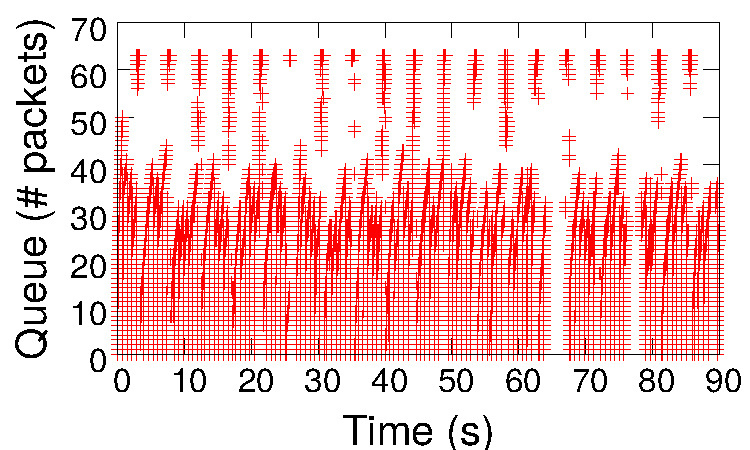
\includegraphics[width=\linewidth]{pq_queue_sizes.pdf}
\vspace{-0.2in}
\caption{Queue depth at egress port 2}
\label{fig:mininet-qin}
\end{subfigure}
\vspace{0.05in}
\caption{Mininet case study measurements.}
\end{figure}
\begin{table}[t]
\centering
\small
\begin{tabular}{|c|c|c|c|c|} \hline
\bf{src $\rightarrow$ dst} & \bf{protocol} & \bf{\# Bursts} & \bf{Time ($\mu$s)} & \bf{\# Packets} \\ \hline
h3:34573 $\rightarrow$ h4:4888 & UDP & 19 & 8969085 & 6090 \\
h4:4888 $\rightarrow$ h3:34573 & UDP & 18 & 10558176 & 5820 \\
h1:1777 $\rightarrow$ h2:58439 & TCP & 1 & 72196926 & 61584 \\
h2:58439 $\rightarrow$ h1:1777 & TCP & 1 & 72248749 & 33074 \\ \hline
\end{tabular}
\caption{Per-flow burst statistics from \TheSystem.}
\label{t:mininet-flowstats}
\vspace{-0.1in}
\end{table}

The results are streamed out on each packet to a collection server. After
plotting the queue latencies, she notices spikes in queue size at egress port 3
on the router (\Fig{mininet-qin}) matching the periodicity of the latency
spikes. To isolate the responsible flow(s), she divides the traffic into
``bursts'', which she defines as a series of packets separated by a gap of at
least 800ms, as determined from the gap between latency spikes. She issues the
following \TheSystem query:

\begin{small}
\begin{lstlisting}
def burst_stats(last_time, nburst, time, pkts, tin):
    if tin - last_time > 800000:
        nbursts++;
        emit();
    else:
        time = time + tin - last_time;
    pkts = pkts + 1;
    last_time = tin;
result = groupby(R1, (*\codeftuple{}*), burst_stats)
\end{lstlisting}
\end{small}

%% NG->Vikram: The burst table is moved to related work to bring it to the head
%% of the next column.

%%\vspace{-0.1in}
She runs the query for 72 seconds and sees the result in
Table~\ref{t:mininet-flowstats}. She concludes, correctly, that UDP traffic
between {\ct h3} and {\ct h4} is responsible for the latency spikes.
There are 18 UDP bursts, with an average size of 320 packets and
average duration of 472 ms, which matches our emulation setup.

\TheSystem's power and flexibility make this diagnosis simple. \TheSystem
allows us to directly instrument a router to reports its own queueing delays
, and flexible
aggregations expose flow statistics (in this case, {\ct burst\_stats}) customized for the problem:
packet counts alone would have disguised the bursty nature of
the offending UDP traffic.

